\cotefile{148}
\scanpage{7}
\mspage{2}

comme l'unique élément de \({}_2(X_S)\) qui
est fixe par $\operatorname{Aut}(X_S)\simeq\mathbb Z/4\mathbb Z$. En fait
\[
\inserted{(X_S)^{\unsure{f}i}\overset{\mathrm{def}}{=}\{x\in X_S\unsure{\deleted{\}}}\mid ix=x\}=\{e,\eta_S\}}
\]
\deleted{\unsure{$X$}} La surface top. $X_S$ a une déc. cell.
\inserted{\unsure{can|ces}} avec 1 sommet $e$, deux arêtes, une face,
\inserted{ces arêtes} correspondant aux deux mailles du réseau $\Gamma_S$.

On considère $X_S$ comme muni de cette décomposition.
Parfois c'est l'image inv. de celle-ci par $2\operatorname{id}_{X_S}$
qui est plus commode, 4 sommets (\unsure{formant|forment} \({}_2(X_S)\)),
\deleted{\unsure{quatre}} \inserted{huit} arêtes,
\deleted{(\uline{NB} \unsure{le}} \inserted{$4^{\unsure{\frown}}$} faces.
On peut considérer $\mathbb Z/4\mathbb Z\simeq\mu_4(\mathbb C)$
comme le groupe d'automorphismes commun de ces deux structures cellulaires.

\figure{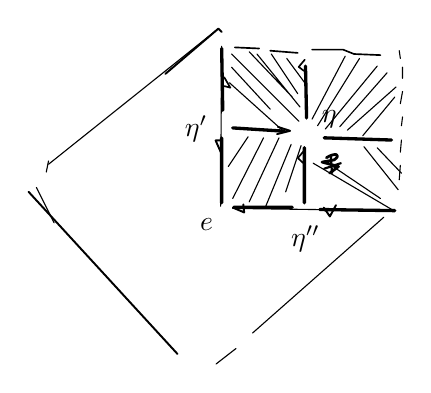
\begin{tikzpicture}[x=.014cm,y=-.014cm,line cap=round,line join=round]
% Detached oblique strokes surrounding the small square.
\draw[thin] (31,143)--(185,20);
\draw[line width=.7pt] (137,61)--(185,20)--(188,23);
\draw[thin] (31,140)--(29,150);
\draw[line width=.7pt] (13,168)--(148,315);
\draw[thin] (20,164)--(36,196);
\draw[thin] (183,324)--(201,310) (216,296)--(335,191);
% Interrupted upper and right edges; exposed left and lower edges.
\draw[thin] (188,36)--(187,181);
\draw[thin] (198,183)--(345,185);
\draw[line width=.6pt] (200,37)--(222,38) (232,40)--(257,42)
 (270,39)--(298,39)--(308,43)--(332,44);
\draw[thin] (349,40)--(350,47) (352,55)--(352,65)
 (352,77)--(350,88) (352,100)--(351,108)
 (351,121)--(350,132) (350,144)--(349,157);
% Heavy portions of the grid.
\draw[line width=1.2pt] (188,38)--(189,94) (188,119)--(188,178)
 (199,182)--(252,182) (277,184)--(345,185)
 (264,54)--(265,101) (263,128)--(263,178)
 (198,110)--(245,113) (281,119)--(342,121);
% Short angular projections on the thick grid strokes; direction remains unassigned.
\draw[line width=.7pt] (188,121.375)--(182.505,121.375)--(188,133.7);
\draw[line width=.6pt] (190.355,72.075)--(195.85,73.525)--(190.355,64.1);
\draw[line width=.7pt] (198.205,182.275)--(208.41,186.625)--(207.625,179.375);
\draw[line width=.7pt] (280.63,182.275)--(286.125,190.25)--(291.62,180.1);
\draw[line width=.7pt] (239.025,109.05)--(250.015,112.675)--(238.24,115.575);
\draw[line width=.6pt] (262.575,130.8)--(257.08,137.325)--(263.36,143.125);
\draw[line width=.6pt] (262.575,58.3)--(257.865,54.675)--(263.36,48.15);
% Hatching, preserving the changing directions.
\draw[thin] (195,69)--(244,113) (197,55)--(232,93)
 (197,43)--(258,104) (213,41)--(252,82)
 (220,43)--(259,91) (233,43)--(257,79) (247,47)--(264,70);
\draw[thin] (270,102)--(300,45) (275,108)--(313,47)
 (282,111)--(329,54) (295,109)--(338,60)
 (302,112)--(346,73) (316,117)--(345,82);
\draw[thin] (194,145)--(212,118) (198,174)--(226,119)
 (213,177)--(240,119) (228,181)--(251,125)
 (246,168)--(260,126);
\draw[thin] (271,142)--(344,185) (286,143)--(332,174)
 (317,127)--(348,166) (329,128)--(351,151);
% Overdrawn cluster below the central junction: no character identification.
\draw[line width=1pt] (283,137)..controls(291,132)and(297,134)..(290,139)
 --(279,141)--(294,145)--(286,151);
\draw[line width=.8pt] (287,135)--(288,151) (281,147)--(296,142);
\node[anchor=north east] at (189,183) {$e$};
\node[anchor=east] at (184,111) {$\eta'$};
\node[anchor=north] at (264,190) {$\eta''$};
\node[anchor=south west] at (270,119) {$\eta$};
\end{tikzpicture}}

Le deuxième est mieux \unsure{adaptée|adapté} pour la description du quotient
\[
\deleted{\unsure{X|X_S}\mathbb E\unsure{\ell|\ell_0}(\unsure{S|2})}\quad X_S/\pm1
\]
qui est une sphère, subdivisée en \deleted{deux} \inserted{faces} \unsure{carrées|carrés},
se raccordant suivant un équateur \deleted{carré}\unsure{,|.}
subdivisé en quatre arêtes par $e^{\unsure{\natural|q}},\eta^{\unsure{\natural|q}},\eta'^{\unsure{\natural|q}},\eta''^{\unsure{\natural|q}}$.

\figure{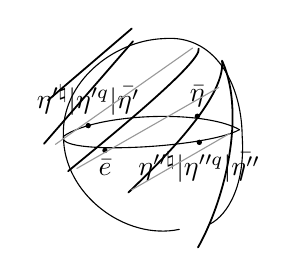
\begin{tikzpicture}[scale=.85,line cap=round,line join=round]
% The outline is interrupted near its lower-right end.
\draw (.45,-1.42)..controls(-.35,-1.59)and(-1.28,-.9)..(-1.28,-.03)
 ..controls(-1.32,.77)and(-.54,1.4)..(.21,1.43)
 ..controls(.98,1.5)and(1.38,.76)..(1.39,-.02)
 ..controls(1.44,-.75)and(1.18,-1.2)..(.91,-1.34);
\draw (-1.28,-.03)..controls(-.8,.31)and(.8,.38)..(1.35,.07);
\draw (-1.28,-.03)..controls(-1.42,-.32)and(.85,-.21)..(1.35,.07);
\fill (-.91,.13) circle (.04);
\fill (.72,.27) circle (.04);
\fill (-.66,-.24) circle (.04);
\fill (.75,-.12) circle (.04);
\node[above] at (-.91,.13) {$\unsure{\eta'^{\natural}|\eta'^{q}|\bar{\eta'}}$};
\node[above] at (.72,.27) {$\unsure{\bar\eta}$};
\node[below] at (-.66,-.24) {$\bar e$};
\node[below] at (.75,-.12) {$\unsure{\eta''^{\natural}|\eta''^{q}|\bar{\eta''}}$};
% Cancellation strokes through the whole drawing.
\draw[line width=.65pt] (-1.51,.51)--(-.26,1.58)
 (-1.57,-.14)--(-.24,1.39)
 (-1.21,-.55)..controls(-.49,.04)and(.79,1.09)..(.74,1.28)
 (-.31,-.87)..controls(.05,-.52)and(1.15,.51)..(1.09,1.1)
 (1.09,1.1)..controls(1.45,.3)and(1.13,-.98)..(.73,-1.69);
\draw[thin,black!40] (-1.4,-.15)--(.65,1.29)
 (-1.08,-.51)--(1.04,.7) (-.26,-.83)--(1.2,.01);
\end{tikzpicture}}

\figure{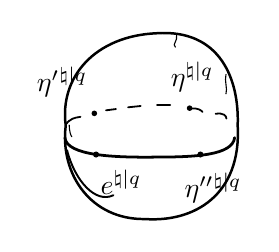
\begin{tikzpicture}[x=.55cm,y=.55cm,line cap=round,line join=round]
\draw[line width=.9pt] (-1.96,.08) .. controls (-2.11,1.20) and (-1.28,2.15) .. (.14,2.21) .. controls (1.61,2.31) and (2.05,1.14) .. (2.01,.08) .. controls (2.10,-1.53) and (1.00,-2.16) .. (-.13,-2.08) .. controls (-1.37,-2.10) and (-2.10,-1.05) .. (-1.96,.08);
\draw[line width=1.0pt] (-1.98,-.20) .. controls (-1.94,-.62) and (-.83,-.66) .. (.09,-.65) .. controls (1.04,-.65) and (1.89,-.61) .. (1.94,-.20);
\draw[line width=.65pt] (-1.96,.10) .. controls (-1.86,.24) and (-1.76,.26) .. (-1.62,.28);
\draw[line width=.65pt] (-1.03,.43)--(-.80,.46);
\draw[line width=.65pt] (-.52,.50)--(-.23,.53);
\draw[line width=.65pt] (.15,.55)--(.45,.55);
\draw[line width=.65pt] (.94,.47) .. controls (1.09,.49) and (1.17,.43) .. (1.20,.39);
\draw[line width=.65pt] (1.50,.35) .. controls (1.69,.38) and (1.75,.30) .. (1.75,.24);
\fill (-1.30,.36) circle (.065);
\fill (.90,.48) circle (.065);
\fill (-1.26,-.59) circle (.070);
\fill (1.15,-.59) circle (.070);
\draw[line width=.7pt] (-1.93,-.49) .. controls (-1.75,-1.20) and (-1.27,-1.73) .. (-.86,-1.53);
\draw[line width=.4pt] (.60,2.18) .. controls (.63,2.02) and (.49,1.96) .. (.57,1.89);
\draw[line width=.4pt] (1.74,1.26) .. controls (1.70,1.10) and (1.78,.94) .. (1.74,.81);
\draw[line width=.4pt] (-1.88,.09) .. controls (-1.88,-.05) and (-1.84,-.16) .. (-1.82,-.18);
\node[above left] at (-1.24,.51) {$\eta'{}^{\unsure{\natural|q}}$};
\node[above] at (.96,.63) {$\eta^{\unsure{\natural|q}}$};
\node[below right] at (-1.38,-.72) {$e^{\unsure{\natural|q}}$};
\node[below] at (1.44,-.78) {$\eta''{}^{\unsure{\natural|q}}$};
\end{tikzpicture}}

\margin{6}

